% =========================================================================== %
% Preamble                                                                    %
% =========================================================================== %

\documentclass[dvipsnames, 12pt]{article}
\usepackage[utf8]{inputenc}

% Set paper geometry
\usepackage[letterpaper, margin=1.87cm]{geometry}

% Must include this before setting title and author
\usepackage{findlay}

\def\bpfcontain{\textsc{BPFContain}}

\title{\Large \bpfcontain: Towards Secure and Usable Containers with eBPF\\{\large COMP5900I Preliminary Work}}
\lhead{\bpfcontain: Towards Secure and Usable Containers with eBPF}

\author{William Findlay}
% For acmart.cls:
%\affiliation{Carleton University}
%\email{williamfindlay@cmail.carleton.ca}

% Add bibliography:
\addbibresource{references.bib}

% To set sans serif font:
%\renewcommand{\familydefault}{\sfdefault}

% =========================================================================== %
% Document                                                                    %
% =========================================================================== %

\begin{document}

% Title page
\maketitle
\thispagestyle{empty}

\vfill
\begin{abstract}
\noindent
Containers are becoming an increasingly important part of the Linux ecosystem.
Containerized package managers like Snapcraft \cite{snap} and FlatPak
\cite{flatpak} enable easy distribution and dependency management for desktop
applications, while Docker \cite{docker} and Kubernetes \cite{kubernetes}
provide a framework for scaling and composing micro-services, especially in the
cloud.  While containers offer a convenient abstraction for distributing and
configuring software, they are also often used as a light-weight alternative to
heavier virtualization techniques, such as virtual machines. Thus, containers
can also be thought of as security mechanisms, implementing a form of isolation
between processes that share the resources of the underlying operating system.

Despite this clear security use case, existing container implementations do not
consider security as a primary goal, and often fall back to insecure defaults
when the host does not support the correct security abstractions. Further,
container security implementations are often complex, relying on a myriad of
virtualization techniques and security abstractions provided by the host
operating system to isolate processes and enforce least-privilege. These
security abstractions often paradoxically require elevated permissions to use in
the first place, resulting in additional security risks when applications are
able to escape confinement.

To rectify these container security issues, I present
\bpfcontain{}\footnote{\bpfcontain{} is a working title and is subject to change in the
future.}, a novel approach to containers under the Linux kernel. \bpfcontain{} is
built from the ground up as a light-weight yet secure process confinement
solution for modern applications. Implemented in eBPF, an emerging technology
for safely extending the Linux kernel, \bpfcontain{} enforces least privilege in
containerized applications without requiring any additional privileges from the
host operating system. Policies are written in a high-level language that is
designed to be readable and modifiable by end-users without requiring
significant security expertise. In this paper, I describe \bpfcontain{}'s design and
implementation, evaluate its performance and security, and discuss how it
compares with existing container solutions.

\end{abstract}
\vfill
\vfill

\clearpage

% Reset page numbering
\pagenumbering{arabic}
\setcounter{page}{1}

% Table of Contents, List of Figures, List of Tables, List of Listings
%\begingroup
%\hypersetup{linkcolor=black}
%\tableofcontents
%\newpage
%\listoffigures
%\newpage
%\listoftables
%\newpage
%\lstlistoflistings
%\newpage
%\endgroup

% Reset page numbering
\pagenumbering{arabic}
\setcounter{page}{1}

% Uncomment for 1.5 spacing:
\onehalfspacing

\section{Introduction}

\todo{Write this.}\footnote{Note for Anil: When you see orange square brackets \todo{like this}, treat them as a todo.}

\section{Background}

\subsection{The Process Confinement Problem}

The \textit{process confinement problem}, also known as the \textit{sandboxing
problem}, refers to the goal of isolating a process or group of processes from
the rest of the running system. In practice, this is often achieved by
restricting an application's possible behaviour to its desired functionality,
specifically targeting its access to security-sensitive system resources such as
files, network interfaces, and other running applications.
Despite decades of work following Lampson's \cite{lampson1973_a_note} first
proposal of the process confinement problem in 1973, process confinement remains
a somewhat open problem to date \cite{crowell2013_confinement_problem}.
\todo{What else do I want to say here?}

%Process confinement is not a new problem---it was first proposed by Lampson
%\cite{lampson1973_a_note} in 1973 and has since been the focus of decades of
%research, both in academia and in industry \cite{saltzer1975_protection, wagner1999_janus, jain05_janus2, crowell2013_confinement_problem, cohen1996_secure, gamble1993_execution_controls, berman1995_tron, goldberg96_janus, provos2003_systrace, kim2013_mbox, findlay20_bpfbox, inoue05_java, bubblewrap, firejail, docker, snap, flatpak}.

\subsection{The Confinement Threat Model}
\label{subsection:threat_model}

To understand why process confinement is a desirable goal in operating system
security, we must first identify the credible threats that process confinement
addresses. To that end, here I describe three attack vectors
(\crefrange{a:1}{a:3}), followed by three attack goals (\crefrange{g:1}{g:3})
which highlight just a few of the threats posed by unconfined processes to
system security, stability, and user privacy.

\begin{enumerate}[label=\bfseries A\arabic*., ref=A\arabic*, labelindent=1em]
    \item \label{a:1} \textsc{Compromised processes.} Unconfined running
    processes have classically presented a valuable target for attacker
    exploitation. With the advent of the Internet, web-facing processes that
    handle untrusted user input are especially vulnerable, particularly as they
    often run with heightened privileges \cite{cohen1996_secure}. An attacker
    may send specially crafted input to the target application, hoping to
    subvert its control flow integrity via a classic buffer overflow,
    return-oriented programming \cite{shacham2007_rop}, or some other means. The
    venerable Morris Worm, regarded as the first computer worm on the Internet,
    exploited a classic buffer overflow vulnerability in the \texttt{fingerd}
    service for Unix, as well as a development backdoor left in the
    \texttt{sendmail} daemon \cite{spafford1989_morris}. In both cases, proper
    process confinement would have eliminated the threat by preventing
    the compromised programs from impacting the rest of the system.

    \item \label{a:2} \textsc{Semi-honest software.} Here, I define semi-honest
    software as that which appears to perform its desired functionality, but
    which additionally may perform some set of unwanted actions without the
    user's knowledge. Without putting a proper external confinement mechanism in
    place to restrict the behaviour of such an application, it may continue to
    perform the undesired actions \textit{ad infinitum}, so long as it remains
    installed on the host. As a topical example, an \texttt{strace} of the
    popular Discord \cite{discord} voice communication client on Linux reveals
    that it repeatedly scans the process tree and reports a list of \textit{all
    applications} running on the system, even when the user has turned off the
    \enquote{display active game} feature\footnote{This feature allows Discord
    to report, in the user's status message, what game the user is currently
    playing. The \enquote{display active game} feature appears to be the
    original motivation behind scanning the process tree.}. This scanning
    behaviour represents a clear violation of the user's privacy expectations.

    \item \label{a:3} \textsc{Malicious software.} In contrast to semi-honest
    software, malicious software is that which is expressly designed and
    distributed with malicious intent. Typically, this software would be
    downloaded by an unsuspecting user either through social engineering
    (e.g.~fake antivirus scams) or without the user's knowledge (e.g.~a drive-by
    download attack). In the case of a computer virus, malicious software may
    replicate itself on the host by infecting other (originally benign) binaries.
    It would be useful to provide the user with a means of running such
    potentially untrustworthy applications in a sandbox so that they cannot
    damage the rest of the system.
\end{enumerate}

\begin{enumerate}[label=\bfseries G\arabic*., ref=G\arabic*, labelindent=1em]
    \item \label{g:1} \textsc{Installation of backdoors/rootkits.} Potentially,
    the most dangerous attack goal in the exploitation of unconfined processes
    is the establishment of a backdoor on the target system.  A backdoor needn't
    be sophisticated---for example, installing the attacker's RSA public key in
    \texttt{ssh}'s list of authorized keys would be sufficient---however, the
    most sophisticated backdoors may result in permanent and virtually
    undetectable escalation of privilege. For instance, a sophisticated attacker
    with sufficient privileges may load a \textit{rootkit}
    \cite{beegle2007_rootkit} into the operating system kernel, at which point
    she has free reign over the system in perpetuity (unless the user manages
    to somehow remove the rootkit or reinstalls the infected operating system).

    \item \label{g:2} \textsc{Information leakage.} An obvious goal for attacks
    on unconfined processes (and indeed the focus of the earliest literature on
    process confinement \cite{lampson1973_a_note}) is information leakage. An
    adversary may attempt to gain access to personal information or other
    sensitive data such as private keys, password hashes, or bank credentials.
    Depending on the type of information, an unauthorized party may not even
    necessarily require elevated privileges to access it---for instance, no
    special privileges are required to leak the list of processes running on
    a Linux system (as in the case of Discord \cite{discord} highlighted above).

    \item \label{g:3} \textsc{Denial of service.} A compromised process could be
    used to mount a denial of service attack against the host system. For
    example, an attacker could take down network interfaces, consume system
    resources, kill important processes, or cause the system to shut down or
    reboot at an inopportune moment.
\end{enumerate}

As shown in the examples above, unconfined processes can pose significant
threats to system security and stability as well as user privacy. The advent of
the Internet has exacerbated many of these threats. Unconfined network-facing
daemons continually process untrusted user input, resulting in an easy and
highly valuable target for attacker exploitation. Email and web browsers have
enabled powerful social engineering and drive-by download attacks, which often
result in the installation of malicious software. Semi-honest software can
violate user expectations of security and privacy by performing unwanted actions
without the user's knowledge. It is clear that a solution is needed to mitigate
these threats---for this, we turn to process confinement.

\subsection{Low-Level Isolation Techniques}
\label{subsection:low_level}

The Linux kernel supports a variety of lower-level abstractions for implementing
virtualization, access control, and enforcing least-privilege. While many of
these mechanisms are insufficient for a full confinement implementation on their
own, they are typically used in \textit{combination} by higher-level techniques
such as containers (c.f.~\Cref{subsection:containers}) to achieve confinement.

\paragraph*{Unix Discretionary Access Control}
\todo{This will be adapted from my literature review}

\paragraph*{POSIX Capabilities}
\todo{This will be adapted from my literature review}

\paragraph*{Namespaces and Cgroups}
\todo{This will be adapted from my literature review}

\paragraph*{System Call Interposition}
\todo{This will be adapted from my literature review}

\paragraph*{Linux Security Modules}
\todo{This will be adapted from my literature review}

\subsection{Containers}
\label{subsection:containers}

\todo{This will be adapted from my literature review}

\subsection{Extended BPF}

\todo{Write this}

\section{\bpfcontain{} Design and Implementation}
\label{sec:design}

Five specific goals informed the design of \bpfcontain{}'s policy language and
enforcement mechanism, enumerated below as Design Goals \ref{d:1} to \ref{d:5}.
%Note that there is a natural interplay between some of these design goals, while
%others are typically perceived as being in contention (specifically usability
%and security). In cases of conflict, it is essential to strike a careful balance
%between each property.

\begin{enumerate}[label=\bfseries D\arabic*., ref=D\arabic*, labelindent=1em]
  \item \label{d:1} \textsc{Usability.}
    \bpfcontain{}'s basic functionality should not impose unnecessary usability
    barriers on end-users.  Its policy language should be easy to understand and
    semantically meaningful to users without significant security knowledge. To
    accomplish this goal, \bpfcontain{} takes some inspiration from other high-level
    policy languages for containerized applications, such as those used in
    Snapcraft \cite{snap}.

  \item \label{d:2} \textsc{Configurability.}
    It should be easy for an end-user to reconfigure policy to match their
    specific use case, without worrying about the underlying details of the
    operating system or the policy enforcement mechanism. It should be possible
    to use \bpfcontain{} to restrict specific unwanted behaviour in a given
    application without needing to write a rigorous security policy from
    scratch.

  \item \label{d:3} \textsc{Transparency.}
    Containing an application using \bpfcontain{} should not require modifying the
    application's source code or running the application using a privileged SUID
    (Set User ID root) binary. \bpfcontain{} should be entirely agnostic to the rest
    of the system and should not interfere with its regular use.

  \item \label{d:4} \textsc{Adoptability.}
    \bpfcontain{} should be adoptable across a wide variety of system configurations
    and should not negatively impact the running system. It should be possible
    to deploy \bpfcontain{} in a production environment without impacting system
    stability and robustness or exposing the system to new security
    vulnerabilities. \bpfcontain{} relies on the underlying properties of its eBPF
    implementation to achieve its adoptability guarantees.

  \item \label{d:5} \textsc{Security.}
    \bpfcontain{} should be built from the ground up with security in mind. In
    particular, security should not be an opt-in feature and \bpfcontain{} should
    adhere to the principle of least privilege \cite{saltzer1975_protection} by
    default. It should be easy to tune a \bpfcontain{} policy to respond to new
    threats.
\end{enumerate}

\subsection{\bpfcontain{} Policy}
\label{sec:policy}

\bpfcontain{} policy consists of simple manifests written in YAML \cite{yaml},
a human-readable data serialization language based on key-value pairs.  Each
\bpfcontain{} container is associated with a manifest, which consists of a few lines
of metadata followed by a set of \textit{rights} and \textit{restrictions}.
A \textit{right} specifies access that should be granted to a container, while
a \textit{restriction} is used revoke access. While rights and restrictions may
be combined at various levels of granularity, a restriction \textit{always}
overrides a right, without exception. In practice, this allows the construction
of nuanced policies that specify coarse-grained access with finer-grained exceptions.
\Cref{tab:accesses} describes the various access labels that can be used in
\bpfcontain{} policy.

\begin{table}[htpb]
  \centering
  \caption{
    A list of accesses supported by \bpfcontain{} policy, along with their
    parameters, if any, and descriptions. Square brackets denote an optional
    parameter.
    \todo{This is currently non-exhaustive, come back and revise.}
  }
  \label{tab:accesses}
  \begin{tabular}{llp{20em}}
  \toprule
  Access              & Parameters              & Description \\
  \midrule
  \texttt{filesystem} & Mountpoint, [Read-only] &
    Grants access at the granularity of a filesystem mountpoint.
    This access may optionally be restricted to read-only. \\
  \texttt{file}       & Pathname, Access        &
    Grants access at the granularity of individual files.
    Access may be specified as read, write, link, delete, or execute. \\
  \texttt{directory}  & Pathname, Access        &
    Grants access at the granularity of individual directories.
    Access may be specified as read, write, link, delete, or chdir. \\
  \texttt{network}    & [Interface]             &
    Grants access to network communications.
    A specific interface may optionally be specified. \\
  \texttt{tty}        & N/A                     &
    Grants access to tty devices. \\
  \texttt{graphics}   & N/A                     &
    Grants access to the graphical server. \\
  \texttt{microphone} & N/A                     &
    Grants access to the microphone. \\
  \texttt{sound}      & N/A                     &
    Grants access to the microphone. \\
  \bottomrule
  \end{tabular}
\end{table}

Following the principle of least privilege \cite{saltzer1975_protection},
\bpfcontain{} implements strict default-deny enforcement, only granting access
that the policy specifically declares under the container's set of rights. The
user may optionally change this behaviour and elect to enforce a default-allow
policy instead, by setting \lstinline[language=yaml]{default: allow} in the
manifest. A default-allow policy enables the easy restriction of specific
unwanted behaviour in a given program, without worrying about the details of
constructing a rigorous security policy.

As a motivating example of \bpfcontain{} security policy, consider the Discord
client, discussed briefly in \Cref{subsection:threat_model}. Discord is a popular
cross-platform voice chat client designed for gamers and comes with an optional
feature, \enquote{Display Active Game}, which displays whatever game the user is
currently playing in their status message. To accomplish this, the Linux Discord
client periodically scans the \texttt{procfs} filesystem to obtain a list of all
running processes.  While this feature may seem innocuous at first glance, an
\texttt{strace} \cite{strace} of Discord reveals that it continually scans the
process tree even when the \enquote{Display Active Game} feature is
\textit{disabled}. This behaviour represents a gross violation of the user's
privacy expectations. To rectify this issue, a user might write a \bpfcontain{}
policy like the examples depicted in \Cref{lst:discord_a} and
\Cref{lst:discord_b}.

\begin{listing}[
  language=yaml,
  caption={
    A sample manifest for Discord \cite{discord} using \bpfcontain{}'s more
    restrictive default-deny confinement. All accesses which are not listed
    under the container's rights are implictly denied. The explicit restriction
    on access to \texttt{procfs} prevents Discord from scanning the process
    tree, regardless of its rights.
  },
  label={lst:discord_a},
  gobble=2]
  name: discord
  command: /bin/discord
  rights:
    - filesystem /
    - network
    - graphics
    - microphone
    - sound
  restrictions:
    - filesystem /proc
\end{listing}

\begin{listing}[
  language=yaml,
  caption={
    A sample manifest for Discord \cite{discord} using \bpfcontain{}'s optional
    default-allow confinement.  This permits a much simpler policy that directly
    targets Discord's \texttt{procfs} scanning behaviour.
  },
  label={lst:discord_b},
  gobble=2]
  name: discord
  command: /bin/discord
  default: allow
  restrictions:
    - filesystem /proc
\end{listing}

In the first example (\Cref{lst:discord_a}), the container grants access to the
root filesystem, networking capabilities, graphical capabilities, microphone,
and sound. It explicitly restricts access to the \texttt{procfs} filesystem,
preventing Discord from scanning the process tree. In the second example
(\Cref{lst:discord_b}), a more permissive policy is defined which serves
\textit{only} to restrict access to \texttt{procfs}. The choice of which
alternative to use is left entirely up to the user, and may depend on various
factors such as the existence of a pre-configured policy file, the desired use
case, and the user's level of comfort with \bpfcontain{}'s policy semantics.

To run a \bpfcontain{} container, the user invokes \texttt{bpfcontain run <name>} where
\texttt{name} is the unique container name declared in the manifest.  The
\texttt{bpfcontain run} command is a thin wrapper around that target application,
whose only purpose is to invoke a special library call,
\lstinline[language=c]|bpfcontain_confine|, that marks the process group for
confinement before executing the command(s) defined in the manifest.

An important feature of \bpfcontain{} is that the
\lstinline[language=c]|bpfcontain_confine| library call requires no additional
operating system privileges to start confinement.  This notion of unprivileged
confinement is a unique advantage over other container implementations in Linux.
Somewhat counter-intuitively, traditional container implementations often rely
on binaries with escalated privileges (e.g.~setuid root) to set up confinement.
Failure to correctly drop these elevated privileges may result in
\textit{escalation of privilege} in the host system, particularly if the
confined process manages to escape the container.  By obviating this need for
elevated privileges, \bpfcontain{} conforms with the principle of least
privilege and improves Linux containers' overall security.

As a side effect of \bpfcontain{}'s design, it is also possible for a generic
application to invoke the \lstinline[language=c]|bpfcontain_confine| library
call directly, eliminating the need to start the target application using the
\texttt{bpfcontain run} wrapper. This notion of self-confinement enables
application developers and package maintainers to ship \bpfcontain{} policy with
their software and enforce it transparently to the end-user. Since \bpfcontain{}
policy is designed to be readable and modifiable by end-users, a security policy
shipped with an application could optionally be tuned by the user according to
their specific needs.

%Besides the fact that it invokes a special library call, there is nothing
%special about the \texttt{bpfcontain run} wrapper---nothing is stopping a typical
%application from invoking \lstinline[language=c]|bpfcontain_confine()| directly, as
%it requires no special privileges. In this sense, one can also think of
%\bpfcontain{} as a mechanism for \textit{unprivileged self-confinement}.
%\Cref{sec:implementation} describes in detail the specifics of how \bpfcontain{}
%implements its confinement mechanism.

\subsection{Architecture}

\bpfcontain{} consists of both userspace and kernelspace components, which
interact co-operatively to implement the containerization and policy enforcement
mechanisms. Roughly, its architecture (depicted in \Cref{fig:architecture}) can
be broken down into the following four components:
\begin{enumerate}[label=\bfseries C\arabic*., ref=C\arabic*, labelindent=1em]

  \item \label{c:1}
  A privileged daemon, responsible for loading and managing the lifecycle of
  eBPF programs and maps, as well as logging security events to userspace.

  \item \label{c:2}
  A small shared library and unprivileged wrapper application used to initiate
  confinement.

  \item \label{c:3}
  A set of eBPF programs, running in kernelspace. These programs are attached to
  LSM hooks in the kernel as well as the shared library in \ref{c:2}.

  \item \label{c:4}
  A set of eBPF maps, special data structures which allow bidirectional
  communication between userspace and kernelspace. These maps are used to track
  the state of running containers and to store the active security policy for
  each container.
\end{enumerate}

\begin{figure}[htpb]
  \centering
  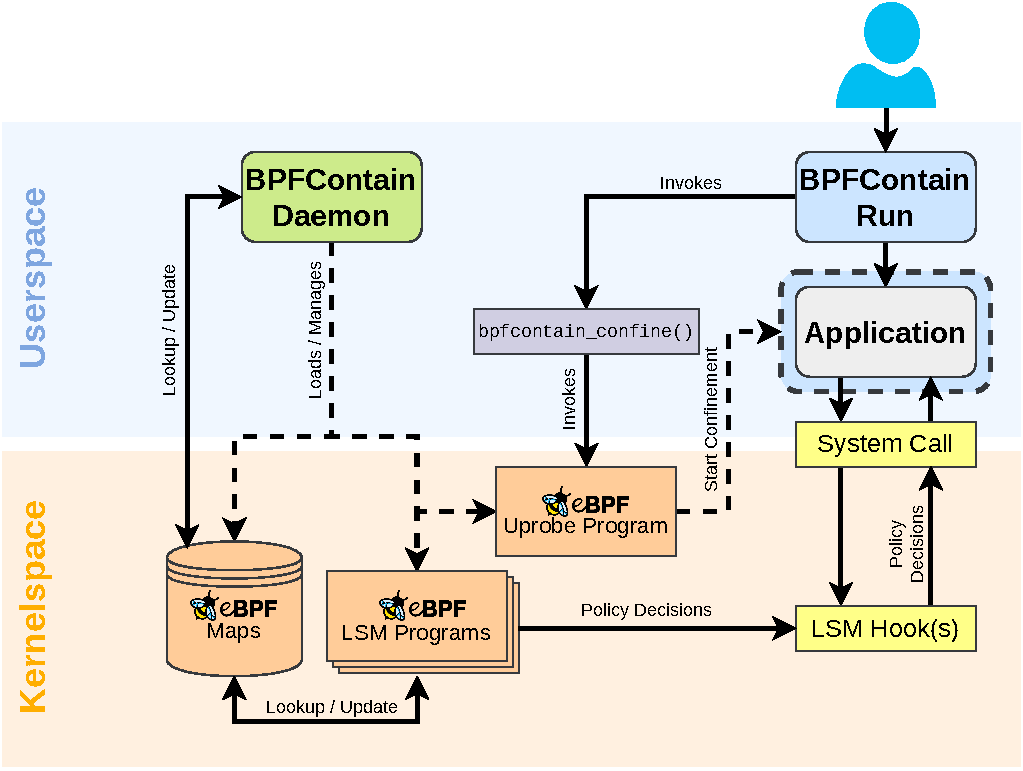
\includegraphics[width=0.8\linewidth]{figs/architecture.pdf}
  \caption{
    A diagram of \bpfcontain{}'s architecture. The privileged daemon (green) is
    responsible for loading the necessary eBPF maps and programs (orange) into
    the kernel and managing their lifecycle. The user starts a container by
    executing an unprivileged wrapper application (blue), which invokes the
    \texttt{bpfcontain\_confine} library call (purple), trapping to a special
    eBPF program that associates the process group with the correct policy.
    When the confined application (grey) makes a system call to request access
    to a sensitive resource, the kernel invokes one or more LSM hooks (yellow)
    which in turn trap to corresponding eBPF LSM programs that make the correct
    policy decision.
  }%
  \label{fig:architecture}
\end{figure}

%\bpfcontain{} consists of several userspace components written in the Python
%programming language and eBPF kernelspace components, written in a restricted
%subset of C.  In userspace, \bpfcontain{} runs a privileged daemon, \texttt{bpfcontain
%daemon}, which is responsible for loading eBPF programs into the kernel,
%creating and managing policy maps, and logging events to userspace. An
%unprivileged helper application, \texttt{bpfcontain run}, is used to run new
%containers.

In userspace, \bpfcontain{} runs in the background as a privileged daemon.  The
daemon is responsible for loading \bpfcontain{}'s eBPF programs and maps and
logging security events to userspace, such as policy violations.  When it first
starts, the daemon invokes a series of \texttt{bpf(2)} system calls to load its
eBPF programs and maps into the kernel. After loading all eBPF programs and
maps, the daemon then parses, translates, and loads each per-container policy
file into specialized policy maps.

To allow processes to request that they be placed into a container,
\bpfcontain{} attaches a specialized eBPF program type called a \texttt{uprobe}
(userspace probe) to a userspace library call, \texttt{bpfcontain\_confine}.
This function is a stub, whose only purpose is to trap to the uprobe---if this
function fails to trap the corresponding eBPF program (for example if
\bpfcontain{} has not yet loaded its eBPF programs into the kernel), this
function returns \texttt{-EAGAIN} to indicate that the caller should repeat the
request. Attaching a \texttt{uprobe} to a library call in this way is a common
eBPF design pattern, which effectively allows eBPF programs to make almost
arbitrary extensions to the kernel's API.

\subsection{Enforcing Policy}
\label{subsection:enforcing}

\todo{Write this}

\section{Evaluation}

\todo{Write this}

\section{Discussion}

\todo{Write this}

\section{Related Work}

\todo{This will be adapted from my literature review.}

\section{Conclusion}

\todo{Write this}

\section{Acknowledgements}

The idea for \bpfcontain{} was conceived during a discussion with Anil Somayaji.
%This work directly builds on my previous work, \textsc{BPFBox}
%\cite{findlay20_bpfbox}, first presented in a paper co-authored with Anil
%Somayaji and David Barrera.

% Uncomment for bibliography:
\clearpage
\printbibliography

\end{document}

% vim:syn=tex
